\section{Introduction}
\label{chp:understanding_understandability}

Search engines are concerned with retrieving relevant information to support a user's information seeking task. Commonly, signals about the topicality or aboutness of a piece of information with respect to a query are used to estimate relevance, with other relevance dimensions like understandability, trustworthiness, etc.~\cite{zhang2014multidimensional} being relegated to a secondary position, or completely neglected. While this may be a minor problem for many information seeking tasks, there are some specific tasks in which dimensions other than topicality have an important role in the information seeking and decision making process. The seeking of health information and advice on the Web by the general public is one such task. 

A key problem when searching the Web for health information is that this can be too technical, unreliable, generally misleading, and can lead to unfounded escalations and poor decisions~\cite{white09b}. Where correct information exists, it can be hard to find and digest amongst the noise, spam, technicalities, and irrelevant information. In \textit{high-stakes search tasks} such as this, access to poor information can lead to poor decisions which ultimately can have a significant impact on our health and well-being~\cite{white09b,white13}. In this work we are specifically interested in the understandability of health information retrieved by search engines, and in improving search results to favour information understandable by the general public. 

The use of general purpose Web search engines like Google, Bing and Baidu for seeking health advice has been largely analysed, questioned and criticised~\cite{graber99,fitzsimmons10,wiener13,patel13,atcherson14,meillier17,ellimoottil12}, despite the commendable efforts these services have put into providing increasingly better health information, e.g., the Google Health Cards~\cite{gabrilovich2016cura}. 

Ad-hoc solutions to support the general public in searching and accessing health information on the Web have been implemented, typically supported by government initiatives or medical practitioner associations, e.g., \url{HealthOnNet.org} (HON) and \url{HealthDirect.gov.au}, among others. These solutions aim to provide \textit{better} health information to the general public. For example, HON's mission statement is ``to guide Internet users to reliable, understandable, accessible and trustworthy sources of medical and health information''. But, do the solutions these services currently employ actually provide this type of information to the health-seeking general public? As an illustrative example, we analysed the top 10 search results retrieved by HON\footnote{Results retrieved on 01/10/2017.} in answer to 300 search queries from CLEF 2016 eHealth (see Section~\ref{sec:data}). Figure~\ref{fig:dist} reports the cumulative distribution of understandability scores for these search results (note, we did not assess their topical relevance). Understandability scores were computed with the most effective readability formula and settings from Section~\ref{sec:which_preprocessing} (Dale-Chall Index). We report also the scores for the ``optimal'' search results (Oracle), as found from  CLEF 2016 (relevant results that have the highest understandability scores), along with the scores for the best retrieval method from Section~\ref{sec:results}. The results clearly indicate that, despite solutions like HON being explicitly aimed at supporting access to understandable health information, they often fail to do so.

In this paper we propose and investigate methods for the estimation of the understandability of health information in Web pages. In doing so, we also study the influence of HTML processing methods on these estimations, and their pitfalls. Then, we investigate how understandability estimations can be integrated into retrieval methods to enhance the quality of the retrieved health information, with particular attention to its understandability by the general public. This paper makes a concrete contribution to practice, as it informs health search engines specifically tailored to the general public about the best methods they should adopt. 

\begin{figure}[t!]
   \centering
   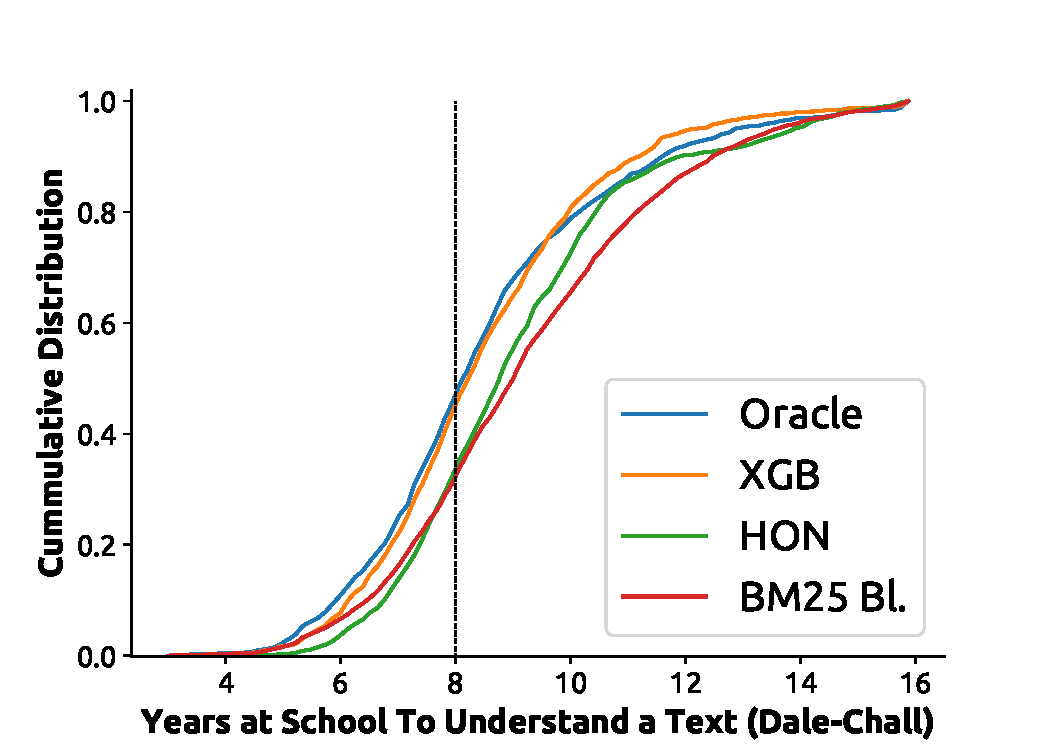
\includegraphics[width=.45\textwidth]{graphics/cumdist}
    \caption{Distribution of Dale-Chall Index (DCI) of search results. DCI measures the years of schooling required to understand a document. The average US resident reads at or below an 8th grade level (dashed line)\cite{cowan04,wallace04,davis04,stossel12}, which is the level suggested by NIH for health information on the Web~\cite{clear94}. The distribution for HON is similar to that of the baseline used in this paper (BM25). Our best method (XGB) re-ranks documents to provide more understandable results; its distribution is similar to that of an ``Oracle'' system.}
   \label{fig:dist}
\end{figure}



%==== ARRIVED TO HERE =====
%
%
%An existing concern of communicators is knowing if their message is well understood by their target public.  
%Writing for a group of readers other than one's own is difficult.
%This fact motived research over the past century on the development of readability formulas which can, through a single number, provide hints on the difficulty of a text.
%Readability formulas were then widely adopted by different groups of the society, showing their effectiveness when increasing the amount learnt by recruits in the army \cite{klare55} or the readership of newspaper \cite{perry54}.
%%became popular and are widely used. For example, different news outlets have are targeting different audiences: TV Guide....NewYorkTimes....
%%....being implemented, for instance, in the Microsoft office package\footnote{\url{https://support.office.com/en-us/article/Test-your-document-s-readability-85b4969e-e80a-4777-8dd3-f7fc3c8b3fd2#ID0EAADAAA=2016,_2013,_2010}}.
%
%Nevertheless, with advent and popularity of Web, in which anyone can write about anything, content has been largely generated without proper concern with its understandability.
%Again: writing for a group of readers other than one's own is difficult and in some domains this might be dangerous.
%The medical domain is one of such \cite{}.
%The problem, as reported by X, is that health consumers might put themselves at risk if they misunderstand the content of what they read on the Web \cite{}.
%Typically health consumers, such as patients and their next-of-kin, start their searches through commercial search engines \cite{}.
%Thus, researchers in various areas of medicine have assessed the understandability of the material retrieved by popular search engines, often finding that they are harder to understand than they should be (e.g., \cite{graber99readability,fitzsimmons2010readability,wiener2013readability,patel13readability,atcherson14readability,meillier17readability}).
%Mostly, this kind of research also relies on the output of readability formulas to deem if a Web page is easy or hard to understand.
%
%However, as recently discussed in Palotti et al.\cite{palotti15}, the automated use of readability formulas firstly requires the content extraction from Web documents.
%Palotti identified that the decision of appending a period at the end of each element in a list or table extracted from the HTML might result either in a single very long or many very short sentences, 
%which drastically affects the interpretation of readability formula results. The same readability formula may yield results that vary from \textit{suitable even for kids} to \textit{understandable only if you are an experts} with only adding or removing a single period, a 'minor' implementation decision when cleaning HTML pages. 
%One limitation of Palotti's work is not evaluating if either of these interpretations is correct.
%
%In this paper, we propose a vast investigation on the preprocessing of Web documents and the correlation of their understandability estimation with human assessments.
%For that, we take advantage of the understandability assessments made in recent Information Retrieval campaigns in CLEF eHealth (\cite{clef15,clef16}).
%
%%\todo{Should we detail the tasks?} 
%During the CLEF eHealth 2015 and 2016 campaigns \cite{clef15,clef16}, organizers explored Internet communities, such as Reddit AskDocs\footnote{\url{https://www.reddit.com/r/AskDocs/}} - in which people seek medical advice free of charge, to generate health consumer searches. Participants in CLEF eHealth campaigns were then instruct to search a considerable portion of the Web\footnote{In 2016 campaing ClueWeb-12 B was used: \url{http://lemurproject.org/clueweb12/}} for documents that could be topically relevant for each consumer query.
%In addition to topical relevance, medical students and health professionals serving as assessors were instructed to assess how easy to understand and how much they would trust the information contained in each assessed document. % The assessment tool used in these campaigns is shown in Figure~\ref{fig:relevation} to enhance the reader understanding.
%%
%In this work, we extensively use the understandability assessments collected in these campaigns.
%%We limit our analysis to the relevant documents to reduce the noise associated with understandability assessments, as the use of ClueWeb-12 B in 2016 campaign resulted in documents from a broad range of topics being retrieved, not only medical ones, and we would like to keep in our analysis only documents related to medicine.
%
%%As also depicted in Figure~\ref{fig:relevation}, understandability assessments were given on a 4-label scale (scores from 0 to 3) in 2015 and on a 0-100 scale in 2016.
%%Easy to understand documents had assessments closer to 0 while hard to understand document had their assessments close to the maximal value, 3 in 2015 and 100 in 2016.
%%Altogether there are 1,452 documents assessed for understandability for CLEF eHealth 2015 and 3,320 for 2016 (see a detailed analysis in Appendix~\ref{apx:clef}, for example, Figures~\ref{fig:boxplot_labels} and~\ref{fig:boxplot_others} report the assessment distribution).
%
%We correlate the human assessments with the output of various readability formulas applied with different preprocessing settings.
%Our first intent is to complete Palotti's work, providing guidelines for the automatic use of these formulas in the Web documents in the medical domain.
%We take advantage of the framework built to further investigate other understandability estimators besides the readability formulas.
%Finally, we use the lessons learnt in our correlation analysis to demonstrate how is possible to retrieve more understandable medical content. 
%
%\todo{add roadmap?}
%
%%We start our experiments in this chapter analysing the correlation of each readability formula to the human assessments, our ground truth, in Section~\ref{sec:which_readability}.
%%We then study other understandability estimators going far beyond the readability formulas. Those are presented in Section~\ref{sec:proxies}.
%%Similarly, to our experiments with readability formulas, we empirically investigate in Section~\ref{sec:beyond_readability} the patterns that lead to effective understandability estimators.
%%In Section~\ref{sec:which_preprocessing} we compare the effect of different preprocessing methods in the light of more than 100 understandability estimators.
%%Our findings and highlights are summarized in Section~\ref{sec:conclusion_doc_analysis}.

